%\begin{savequote}[8cm]
%Alles Gescheite ist schon gedacht worden.\\
%Man muss nur versuchen, es noch einmal zu denken.

%All intelligent thoughts have already been thought;\\
%what is necessary is only to try to think them again.
 % \qauthor{--- Johann Wolfgang von Goethe \cite{von_goethe_wilhelm_1829}}
%\end{savequote}

\chapter{\label{ch-FurtherSims} Further simulation campaigns in the low-CR regime}

\minitoc

\section{Introduction}
The previous chapter had three key results. Firstly, this new expected low-instability regime was defined, where 1D simulation is expected to provide a reasonable estimate of performance. Secondly, the performance of conventional hot-spot implosions of wetted-foam capsules using third-harmonic laser light was explored and well-characterised. Finally, the code and methodology for this style of optimisation campaign was established.

In this chapter, these previous results will be built upon through further simulation.  In \hl{SECTION}, the impact of the EOS model used to describe the wetted-foam is investigated, in an attempt to address one of the limitations noted at the end of the previous chapter. One of the other limitations mentioned of this approach was the difficulty of verifying this regime experimentally, and so in \hl{SECTION} a new surrogate target (the `hydrodynamic equivalent' capsules) are proposed and optimised to allow room temperature experiments.

In the second half of the chapter, further simulation campaigns are performed to explore how new techniques could be applied within the low-instability regime to further increase fusion performance. In \hl{SECTION} the potential performance benefits of using higher frequency lasers are investigated, through additional implosion optimisations. Finally, in section \hl{section}, an auxiliary heating scheme using electron beams is discussed and applied to the previous simulations.

\subsection{An alternative fusion metric: the burning plasma parameter}
It is relevant at this stage to introduce an additional fusion metric, which will be used later in this chapter (in particular in \hl{Section}) to evaluate fusion performance. So far in this thesis gain has been the primary fusion metric, but this measure of performance has some limitations for this particular work. Gain requires the input energy of the implosion to be known, which this is not the case in \hl{Section} where the energy required to cause the simulated heating is not known to high accuracy. This dependence on input energy means that an identical implosion will therefore appear more/less successful in terms of gain depending on the efficiency with which it can be driven. As such, it is useful to introduce alternative metrics that do not suffer from this.

Therefore, a metric known as the `burning plasma parameter' is used. The version used here - the `total capsule burning plasma parameter' - is defined as 
\begin{equation} Q^\mathrm{{tot}}_{\mathrm{\alpha}} = \frac{1}{2} \frac{E_\mathrm{\alpha}}{ E^\mathrm{{tot}}_{\mathrm{PdV}}}, \label{eqn:Qtot defn} \end{equation} where $E_\mathrm{\alpha}$ is the alpha particle energy deposited back into the hotspot over the total duration of the implosion, and $E^\mathrm{{tot}}_{\mathrm{PdV}}$ is the total work done on the capsule hotspot and shell at the time of stagnation (maximum pressure) \cite{Betti2015}. This metric compares the energy absorbed from alpha self heating at the bang time of the capsule to the external energy used to compress the capsule; the burn is assumed to be symmetric around the bang time, such that the alpha self-heating at the bang time is equal to half of the total alpha heating $E_\mathrm{\alpha}$ (explaining the factor half in the formula). 

A value of $Q^\mathrm{{tot}}_{\mathrm{\alpha}} > 1$ defines the `burning plasma' regime, where more alpha heating is the dominant source of energy in the capsule \cite{Christopherson2020}. The burning plasma parameter is therefore a useful metric for fusion capsules, as it provides direct information about the energetics of the implosion. It does not depend on input energy, and thus how efficiently the capsule is driven; this makes it ideal for analysing the auxiliary heating capsule, as unlike gain it is not influenced by factors such as how efficiently the electron beams could be generated (which are independent of the implosion).

An early rough indicative estimate for ignition based on the burning plasma parameter was set at $Q^\mathrm{{tot}}_{\mathrm{\alpha}} = 10$, where the cumulative alpha heating at the bang-time is ten times greater than the work done on the hot spot and shell \cite{Betti2011}. However, it should be noted that there is a subtly different variant of the burning plasma parameter, known as the `hotspot burning plasma parameter', where the total work done on the whole capsule $E^\mathrm{{tot}}_{\mathrm{PdV}}$ is instead replaced by the total work done on the hotspot only, and the value is typically around twice as large \cite{Betti2015}. An alternative ignition criteria has been proposed based on this parameter \cite{Christopherson2020}, where $Q^\mathrm{{hs}}_{\mathrm{\alpha}} > 1.4$ is treated as the threshold. This definition treats ignition as the the point at which self-heating results in burn propagation through the cold shell (demonstrating the ambiguity surrounding ignition discussed in \hl{Section}).

\section{Hydro-equivalent capsules}
The capsules described in the previous chapter use cryogenic capsules, and operate with a direct laser drive. At the time that this work was performed this presented a major barrier to experimental verification of this work, as there were no facilities that operated at the high (0.8 and 1.7 MJ) energy scales proposed that could conduct direct-drive shots of cryogenic targets \cite{Hohenberger2015}. Recent developments since this work was performed have addressed this and wetted-foam PDD shots are now planned for the NIF, but the relative scarcity of cryogenic NIF shots makes alternative ways of verifying such work experimentally remain useful. As such, potential surrogate `hydrodynamic equivalent' or `hydro-equivalent' versions of these implosions were developed (following in the footstep of previous surrogate experiments using symmetry capsules to study hydrodynamic behaviour \cite{Weber2016}). 

Here, the cryogenic DT-wetted foam layer is replaced with a dry foam (without DT-wetting) of equivalent density, removing the need for cryogenic cooling. This change is demonstrated in Figure \ref{fig:Hydroequivalent}. In the original capsule, the wetted foam layer consisted of a low density foam ($\sim$25~\si[per-mode=symbol]{\milli\gram\per\centi\meter\cubed}) saturated with liquid DT, giving an overall layer density of 253~\si[per-mode=symbol]{\milli\gram\per\centi\meter\cubed}. In the new capsule this layer is replaced with a higher-density 253~\si[per-mode=symbol]{\milli\gram\per\centi\meter\cubed} foam, without any DT, to leave the overall layer density  unchanged. Other than the density and presence/absence of DT, the foam used in the two capsules is equivalent.

\begin{figure} 
\centering     %%% not \center
\subfigure a){\label{fig:280Cap}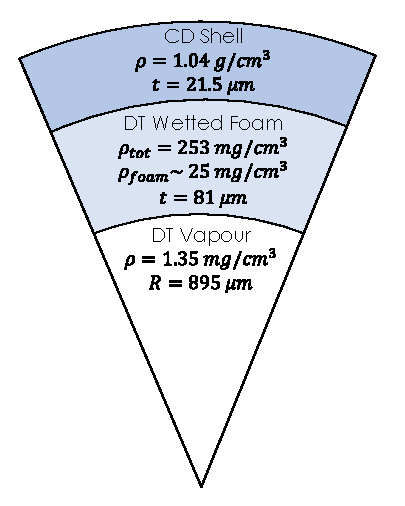
\includegraphics[width=.35\textwidth]{figures/LowCR/280Capsule.pdf}}
\subfigure b){\label{fig:280Hydro}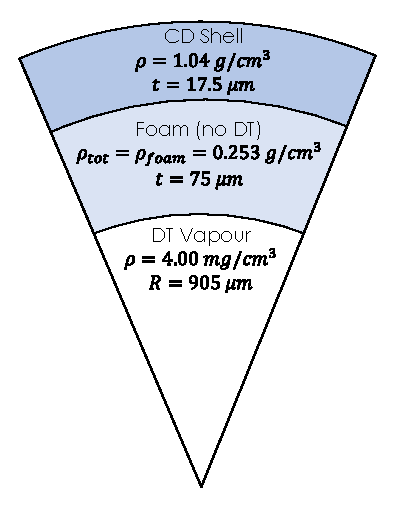
\includegraphics[width=.35\textwidth]{figures/LowCR/280Hydro.pdf}}
\caption{\label{fig:Hydroequivalent} a) The original 280 kJ wetted foam capsule. b) The 280 kJ hydroequivalent capsule. A higher foam density is used to compensate for the lack of DT, to give an equivalent layer density. The optimisation process if then reran, resulting in slightly different laser timings and layer thicknesses.}
\end{figure}

Hydro-equivalent versions of three different implosions have been developed, and are displayed (and compared to the original designs on which they are based) in Table \ref{tab:Hydroequivalent}. In each case, the new capsule was optimised according to the same optimisation procedure used in the previous chapter, maximising the gain of the implosion while satisfying the four criteria. In each case, this results in an implosion with much reduced yield and gain (due to the significantly reduced quantity of DT). However, the key hydrodynamic variables used to define the low instability regime - the convergence ratio, IFAR, and implosion velocity - are very similar to the original capsules, and continue to satisfy the low-instability criteria.

\begin{table}
\resizebox{\textwidth}{!}{%
\centering
\begin{tabular}{|c|c|c|c|c|c|c|}
\hline
Size multiplier &  \multicolumn{2}{c|}{0.35} & \multicolumn{2}{c|}{0.5} & \multicolumn{2}{c|}{0.65} \\ 
\hline
Hydroequivalent? & - & H.E. & - & H.E. & - & H.E.  \\
\hline
Laser energy (MJ) & 0.27 & 0.24 & 0.77 & 0.78 & 1.7 & 1.5 \\ 
Gain &  0.067 & 0.0094 & 0.19 & 0.016 & 0.75 & 0.023\\ 
Convergence ratio & 15.7 & 16.0 & 16.0 & 16.0 & 15.8 & 15.8 \\ 
IFAR & 27.5 & 28.4 & 29.7 & 29.4 & 25.1 & 29.3 \\ 
Implosion velocity (km/s) & 395.8 & 396.3 & 399.6 & 388.9 & 399.6 & 387.5\\ 
Max pulse power (TW) & 84.79 & 84.79 & 173.00 & 173.00 & 292.38 & 292.38\\ 
Pulse 2 switch on time (ns) & 2.20 & 2.70 & 2.60 & 2.50 & 3.60 & 3.70\\ 
Pulse 3 switch on time (ns) & 4.60 & 4.90 & 5.60 & 5.90 &7.80 & 7.80\\ 
Pulse 4 switch on time (ns) & 5.50 & 5.80 & 6.80 & 6.90 & 9.50 & 9.20 \\ 
Laser switch off time (ns) & 8.50 & 8.50 & 11.00 & 11.20 & 15.00 & 14.20 \\ 
Vapour/liquid boundary (\si[per-mode=symbol]{\milli\meter}) & 0.8950 & 0.9050 & 1.3050 & 1.3150 & 1.6705 & 1.7225\\ 
Liquid/CD boundary (\si[per-mode=symbol]{\milli\meter}) & 0.976 & 0.980 & 1.3950 & 1.3950 & 1.8200 & 1.8135\\ 
Outer radius (\si[per-mode=symbol]{\milli\meter}) & 0.9975 & 0.9975 & 1.4250 & 1.4250 & 1.8525 & 1.8525\\ 
Vapour density (\si[per-mode=symbol]{\milli\gram\per\centi\meter\cubed}) & 1.35 & 4.00 & 1.05 & 3.90 & 1.00 & 3.75\\
\hline
  \end{tabular}}
  \caption{Hydroequivalent implosions for three capsule size. The wetted foam implosion for each size has been included for comparison. All implosions use a four-pulse laser sequence. The hydroequivalent capsules have been optimised, resulting in slightly different values for the optimisation parameters and the laser energy, but the hydrodynamic parameters are broadly similar.}
  \label{tab:Hydroequivalent}
\end{table}

This provides a series of surrogate capsules, which could be used in room temperature experiments to validate this regime and verify the assumptions of low instability growth. These capsules could be shot, the amount of instability growth quantified, and their performance compared to the 1D simulations. If the instability growth is low and the agreement with the simulations good, then this would suggest that the four criteria used to define this regime are indeed sufficient to guarantee good agreement, and thus that the designs presented in the previous chapter would likely perform with similar agreement. 

\section{Mixed foam EOS studies}






\section{Alternative laser drivers}

A possible way to increase fusion performance is to increase the frequency of the laser driver. Higher frequency lasers have have a higher energy coupling with the plasma, which results in a greater ablation pressure for equivalent laser intensity. The higher frequency also has a higher critical density and can thus propagate further into the plasma, leading to increased laser absorption (since the light travels through more material) and a higher density blow-off \cite{Obenschain2020}. The lower laser wavelength also means that higher intensities are permitted before the onset of significant parametric instability growth \cite{Montgomery2016} (as highlighted by the $I \cdot \lambda^2$ criteria for the low-instability regime). 

The simulation platform described in the previous section is well-suited to an investigation of different laser drivers. The laser frequency can easily be changed in the Hyades input decks, and the same style of optimisation campaign can then be performed. The purpose of doing such is two-fold: the possible performance in the low-instability regime is further investigated, and the possible impact of increasing the laser driver can be investigated, quantified, and compared to the third-harmonic simulations in the previous section (all in a regime where reasonable agreement is expected between experiment and simulation). Two different laser drivers are considered in this section: a 193 \unit{\nano\meter} laser with a similar pulse profile to the previous simulations, and a novel `two-colour' laser driver.

\subsection{Background to possible IFE laser drivers}

Designs for IFE power plants have a number of requirements, including high laser efficiency, broadband laser operation, and (obviously) high gain. There are two main laser technologies that are seen as potentially satisfying these requirements; diode-pumped solid-state lasers (DPSSL) and electron-beam pumped excimer lasers, such as KrF or ArF \cite{Craxton2015}. 

The DPPSL fundamental wavelength is 1.05 \unit{\micro\meter}, which can be frequency tripled to 0.35 \unit{\micro\meter} - the same frequency used at the NIF, and thus that the previous simulations were performed for. The DPSSL technology is similar to that used at the NIF, where flash lamps are used to pump a solid state glass gain medium; but for DPSSL, the flashlights (which are inefficient, as they emit broadband light) are replaced with diode lasers which pump the medium at the appropriate frequency much more efficiently \footnote{the gain medium is not necessarily the same Nd:glass medium currently used at the NIF, but this is an option under consideration}. 

Excimer lasers are naturally higher frequency, with fundamental wavelengths of 0.258 \unit{\micro\meter} for KrF lasers and 0.193 \unit{\micro\meter} for ArF lasers. In excimer lasers, the gain medium is a gaseous mixture of a noble gas (Kr or Ar) and a halide (F). An electrical discharge is driven through the medium to excite it, leading to the formation of exciplex molecules - these emit UV radiation when they relax, and it is this relaxation which is used to provide the laser emission. There have been a number of excimer lasers developed (including Sprite/Titania at the CLF \cite{Divall1996}, Garpun at Lebedev Physical Institute \cite{Zvorykin2006}, and Nike at the NRL \cite{Obenschain1996}), but these have so far been limited to energies below 10 kJ. 

The `high average power laser' programme conducted between LANL and NRL investigated future laser drivers for IFE power-plants, and led to the development of high repetition rate lasers based on the two technologies \cite{Craxton2015}; the Electra KrF laser at the NRL (which could produce energies of up to 700 J and repetition rates of up to 5 Hz), and the Mercury DPSSL laser an LANL (which gave shots greater than 50J, with a repetition rate of up to 10 Hz \cite{Sethian2010}. Both lasers performed well, and this led to the conclusion that either technology could be viable for an IFE power plant and development of both approaches should be pursued.

Both approaches have their advantages. DPSSL lasers are likely more robust (as they are entirely solid-state), and the lower fundamental frequency is beneficial for preventing damage to laser optics \cite{Sethian2010}. However, excimer lasers have some strong advantages for direct-drive fusion performance. This includes the higher frequency (and thus greater laser absorbiton), but also a very smooth beam profile (desirable for direct-drive), good capability for focal zooming, and an inherently high bandwidth (significant for preventing parametric instability growth). These properties mean that simulations suggest that KrF or ArF lasers could be used to achieve higher gains for equivalent energies to DPSSL lasers. There is therefore a continuing interest in these technologies, as demonstrated by recently published simulations suggesting significant gains at low energies using ArF lasers for shock ignition \cite{Obenschain2020}.

\subsection{ArF lasers}

The optimisation procedure described in the previous chapter was repeated for a series of capsule sizes, but the laser frequency within the simulations was changed from the third-harmonic of Nd:glass to the 193~nm - the fundamental frequency of an ArF laser, and the same frequency used for the previously mentioned shock-ignition simulations \cite{Obenschain2020}. This can be easily achieved simply by changing the frequency in the HYADES input decks. In the low instability-regime outlined in the previous chapter, the maximum permitted laser power is set by a limit on $I \cdot \lambda^2$; increasing the frequency thus meant that the laser power could also be increased, while continuing to satisfy this criteria. All the laser powers were thus scaled accordingly. 

Other than the change to the laser frequency and the laser pulse powers, the simulation campaign was identical. The same capsule structure and four-pulse laser sequence was used, with the same seven optimisation parameters. This new campaign therefore is used to investigate the performance that could be achieved within the low-instability regime using an ArF laser. However, as the changes depend only on the frequency, this is used to demonstrate more broadly how moving to higher frequencies generally - be that from using a KrF laser (0.258 \unit{\micro\meter}), or using the fourth (0.263 \unit{\micro\meter}) or fifth (0.210 \unit{\micro\meter}) harmonic of Nd:glass - would influence the performance.

Three different capsule sizes were simulated and optimised by two summer students (Heath Martin and Rusko Ruskov) under my supervision. I provided the code required to do the simulation campaign, adjusted this to provide simulations at the new frequency with the new pulse powers, and then trained and supervised the two students as they performed the simulations. The tabulated results are displayed in \ref{tab:TwoColourTable}, and are plotted in \ref{fig:ArF and Two colour}.

\begin{figure}[ht]
\centering
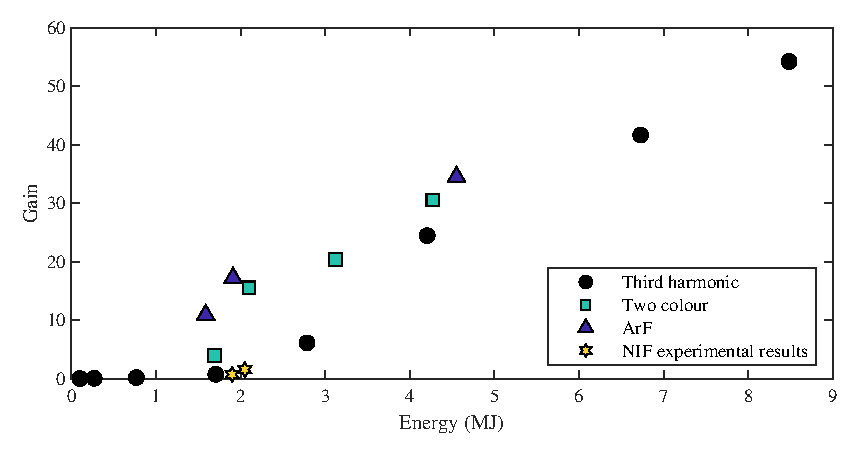
\includegraphics{figures/FurtherSims/ArFandTwoColour.eps}
\caption{A plot of the gain vs the laser energy for simulations using the three different laser drivers. The NIF 210808 experimental shot, and the recent NIF ignition shot, have been included for comparison.}
\label{fig:ArF and Two colour}
\end{figure}

\begin{table}
\resizebox{\textwidth}{!}{%
\centering
\begin{tabular}{|c|c|c|c|c|c|c|c|}
\hline
Laser driver   & \multicolumn{3}{c|}{ArF} & \multicolumn{4}{c|}{Two-colour} \\ 
\hline
Size multiplier & 0.45 & 0.5 & 0.65 & 0.5 & 0.65 & 0.75 & 0.85 \\
\hline
Total laser energy (MJ)  & 1.59 & 1.91 & 4.55 & 1.69 & 2.10 & 3.12 & 4.27\\ 
3rd harmonic energy (MJ) & - & - & - & 0.92 & 1.82 & 2.75 & 3.96 \\
ArF energy (MJ)  & 1.59 & 1.91 & 4.55 & 0.77 & 0.28 & 0.37 & 0.32\\
Gain & 10.9 & 17.3 & 34.5 & 4.0 & 15.5 & 20.4 & 30.5 \\ 
Convergence ratio  & 16.0 & 15.9 & 14.0 & 16.0 & 16.0 & 16.0 & 16.0\\ 
IFAR  & 11.3 & 10.5 & 8.5 & 16.1 & 20.4 & 23.8 & 23.4 \\ 
Implosion velocity (km/s)  & 390.7 & 398.9 & 360 & 391.1 & 399.9 & 396.4 & 391.6\\ 
Max 3rd harmonic power (TW)  & - & - & - & 173 & 292 & 389 & 500\\
Max ArF laser power (TW)  & 464 & 572 & 967 & 274 & 463 & 617 & 792\\ 
Pulse 2 switch on time (ns)  & 3.90 & 3.50 & 2.50 & 1.95 & 3.00 & 2.70 & 3.50\\ 
Pulse 3 switch on time (ns)  & 7.10 & 7.50 & 8.90 & 4.35 & 7.80 & 7.20 & 9.10\\ 
Pulse 4 switch on time (ns)  & 8.85 & 9.25 & 10.80 & 8.05 & 9.40 & 9.10 & 11.10\\ 
2nd laser switch on time (ns)& - & - & -  & 10.00 & 14.70 & 15.20 & 18.20 \\
Laser switch off time (ns)  & 11.95 & 12.25 & 15.10 & 12.80 & 15.30 & 15.80 & 18.60\\ 
Vapour/ice boundary (\si[per-mode=symbol]{\milli\meter})  & 1.072 & 1.210 & 1.435 & 1.230 & 1.645 & 1.933 & 2.210\\ 
Ice/CD boundary (\si[per-mode=symbol]{\milli\meter})  & 1.200 & 1.340 & 1.780 & 1.360 & 1.818 & 2.100 & 2.374\\ 
Outer radius (\si[per-mode=symbol]{\milli\meter}) & 1.2800 & 1.425 & 1.8525 & 1.425 & 1.8525 & 2.1375 & 2.4225 \\ 
Vapour density (\si[per-mode=symbol]{\milli\gram\per\centi\meter\cubed})& 1.00 & 1.03 & 0.60  & 1.02 & 1.05 & 1.00 & 1.01 \\
\hline
  \end{tabular}}
  \caption{Simulation parameters for the two-colour and high frequency implosions.}
  \label{tab:TwoColourTable}
\end{table}

It can be seen in Figure \ref{fig:ArF and Two colour} that the ArF implosions display a significant improvement in gain for a given energy compared to the previous third-harmonic simulations. A gain of 11 can be achieved for around 1.6 MJ of laser energy, which is an order of magnitude higher than is predicted using third-harmonic. This clearly displays the potential benefits of using a higher frequency laser driver. It should again be noted that this is in the low-instability regime, and thus it should be expected that instability growth would be minimal and 1D simulations should give a reasonable estimate of performance.

The physical properties of these implosions should also be commented on. For an ArF implosion the laser power is much higher compared to a third-harmonic implosion, but the limit on implosion velocity means that the implosion takes a similar amount of time. This means that the ArF implosion for a given capsule size has a much higher laser energy than an equivalently sized third-harmonic capsule (or alternatively, for the same energy the ArF implosion will use a smaller capsule). In terms of fusion performance, using a higher laser frequency has essentially shifted the ignition curve to lower energies; the capsule fuel mass has not changed, and so if the laser energy was allowed to increase indefinitely the yield would saturate at the same value. Rather, the ArF laser allows more favourable temperatures and densities to be achieved at a given energy, meaning that the onset of fusion reactions (and thus ignition) occur at lower energies. 

\subsection{Two-colour implosions}

Higher frequency lasers (whether excimer or higher harmonics of Nd:glass) are less technologically developed than third-harmonic Nd:glass lasers, and have not yet been demonstrated at such high energies. This makes the previous ArF results challenging to achieve in practice. As such, an alternative driver-scheme is proposed, where the higher frequency laser is used to supplement a third-harmonic driven implosion. This still requires much larger high frequency laser energies than are currently available, but it is a significant reduction compared to the previous simulations. The new scheme is a compromise solution, allowing some of the performance benefits of the higher frequency laser to be realised, without requiring such a large laser based on this novel technology. This concept will be referred to as a `two-colour' approach.

The laser scheme proposed is shown in figure \ref{fig:Two colour sequence}. A four-pulse third-harmonic sequence is applied, of the with the same pulse-profile as used in the previous simulation campaigns. Then, at a late stage in the implosion, a high-power short-duration pulse is applied at the higher ArF laser-frequency. While the four-pulse sequence was already at the maximum allowed power under the $I \cdot \lambda^2$ criteria, the lower wavelength of the final pulse means a higher power can be tolerated. The $I \cdot \lambda^2$ criteria is applied separately for the two lasers, given the large separation in wavelength between them (it has been demonstrated previously that using multiple frequencies leads to lower instability growth \cite{Follett2018}).

\begin{figure}[ht]
\centering
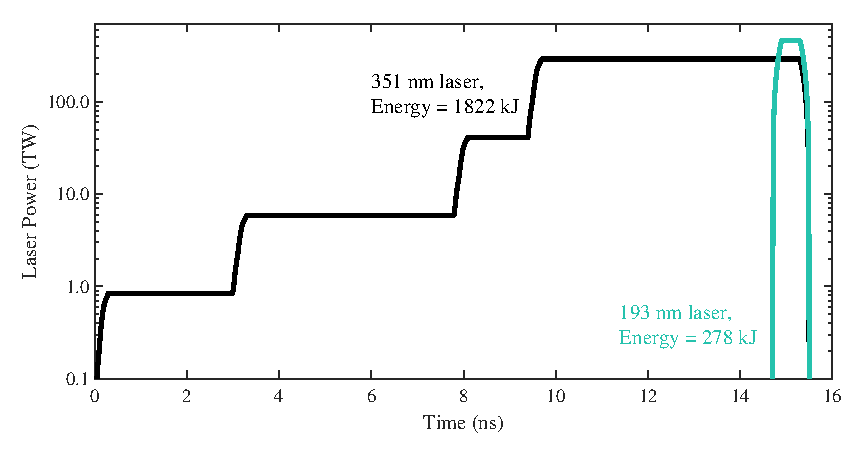
\includegraphics{figures/FurtherSims/TwoColourLaser.eps}
\caption{A log plot of laser power vs time for the 0.65 size two-colour implosion (which achieves a gain of 15.5). A four-pulse third harmonic laser is applied, which is supplemented by a single late pulse from an ArF laser. The ArF has a higher frequency, and thus a higher peak power can be used than for the third harmonic laser.}
\label{fig:Two colour sequence}
\end{figure}

As before, the four criteria for the low-instability regime continued to be applied. In particular, this meant that the implosion velocity was still unable to increase past 400 \unit{\kilo\meter\per\second} at any point in the implosion. This meant that heavier (thicker) shells were used which were accelerated to lower velocities by the third-harmonic laser, so that they continued to remain under the 400 \unit{\kilo\meter\per\second} limit once the high-frequency pulse has been applied. The addition of a late pulse made the optimisation more challenging, as it added an additional optimisation parameter (the switch on time of the final pulse). A  lower maximum ArF laser power was used for the late pulse than the maximum permitted under the $I \cdot \lambda^2$ constraint, or than was used for the ArF-frequency implosions; this appeared to be beneficial in preliminary simulations, but the more challenging optimisation procedure meant this parameter was not investigated further. 

Four two-colour implosions were optimised. I wrote the code to allow this new simulation campaign to be conducted/analysed and performed some preliminary simulations, with the main optimisation campaign then again performed by Heath Martin and Rusko Ruskov under my supervision. The results are displayed alongside those of the ArF simulations in \ref{tab:TwoColourTable}, and are plotted in \ref{fig:ArF and Two colour}.

It can be seen that, as expected, the results for the two-colour implosions consistently fit somewhere between those of the third-harmonic and ArF-frequency results. At 1.7 MJ, the two-colour sequence results in a gain of 4; lower than the gain of 11 achieved for a 1.6 MJ ArF sequence, but a significant improvement compared to the gain of 0.8 achieved using third-harmonic driver. Perhaps more significant is the gain of 15.5 achieved at 2.1 MJ, requiring only 280 kJ of the high-frequency laser. While still a significant increase over current energies for these lasers, this provides a clear demonstration of how this technique leads to significant increases in gain for much more moderate amounts of high-frequency laser energy; although it should be noted that this scheme would require a facility where the capsule can be irradiated uniformly using two different frequencies at the same time \footnote{This approach would therefore perhaps be more suited to higher harmonics of Nd:glass rather than an ArF laser, as then a single laser system could be used with the higher frequency provided by further frequency conversion on some of the beams}.

There are other features of this implosions that it is interesting to comment on. First, note the variation in the proportion of the total energy within the late pulse. This is likely a result of the difficulty in optimising these sequences, due to the additional optimisation parameter. These results are intended only as an initial investigation of this approach, but it appears that it may be possible to gain increased performance with further optimisation. Also, the low IFAR values of these implosions should also be noted, highlighting that this increased performance is achieved by accelerating thicker shells compared to the third-harmonic implosion. Some caution is required here when predicting the amount of Rayleigh-Taylor growth based on the IFAR value, due to the fact that the IFAR quoted corresponds to that measured when the capsule shell is at two thirds of the initial capsule radius. This is before the late-pulse is applied, and thus the IFAR value contains no information about the effect of this late pulse. Trends between the IFAR value and the amount of instability growth are based on experiments and theory which do not include the impact of this late pulse, and thus do not necessarily apply in the same way to the two-colour approach. However, low-instability growth is still predicted, due to three reasons: 1) the IFAR values are low even compared to the criteria of 30, allowing for some further compression of the shell; 2) the three additional criteria also serve to minimise instability growth; and 3) as the additional pulse is applied late, there is less time for any instabilities that it potentially seeds to grow. If this approach were to be pursued, these predictions should be tested with two-dimensional simulations.

\subsection{The burning plasma parameter for alternative laser drivers}

The burning plasma parameter for all of the implosions shown in Figure \ref{fig:ArF and Two colour} has been calculated\footnote{The terms were evaluated as follows: 1) the total work done $E^\mathrm{{tot}}_{\mathrm{PdV}}$ was evaluated as the sum of hotspot and shell kinetic and thermal energies, at the point during the deceleration of the shell where these two energies are equal. This corresponds to a period where the total energy of the capsule is constant, just prior to the onset of fusion reactions. 2) the deposited alpha energy over the full capsule was used rather than the hotspot for $E_\mathrm{\alpha}$, assuming that this absorbtion is dominated by the hotspot \cite{Christopherson2018}. These quantities were evaluated in this way to reduce the dependence of the calculated quantity on the exact position of the hotspot interface, so that it was more robust to issues with hotspot tracking.}, using Equation \ref{eqn:Qtot defn}. The ArF and two-colour implosions can all be seen to be well within the burning-plasma regime, with burning plasma parameters of around 10 and above. It can be seen that the 1.7 MJ third-harmonic implosion is the first third-harmonic result to achieve burning plasma.

\begin{figure}[ht]
\centering
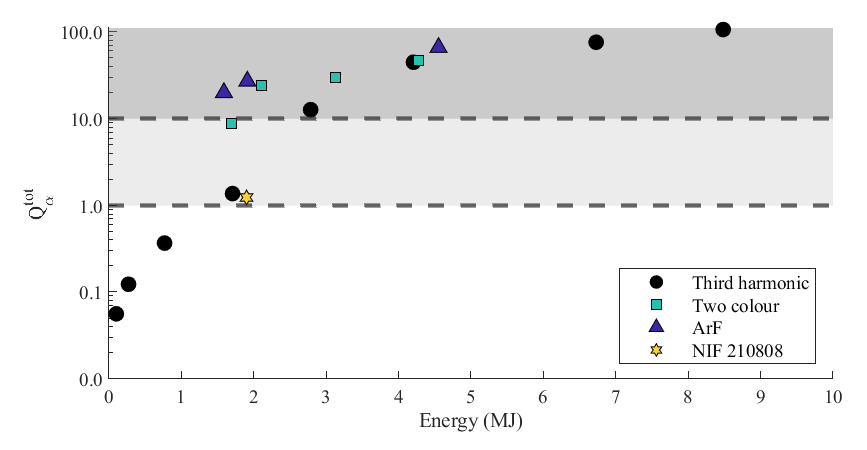
\includegraphics{figures/FurtherSims/QTwoColour.eps}
\caption{A log plot of the total capsule burning plasma parameter $Q^\mathrm{{tot}}_{\mathrm{\alpha}}$ vs laser energy for the optimised capsules using the three laser drivers. Values of $Q^\mathrm{{tot}}_{\mathrm{\alpha}} = 1$ and $Q^\mathrm{{tot}}_{\mathrm{\alpha}} = 10$ are indicated.}
\label{fig:TwoColourQ}
\end{figure}

NIF shot data for N210808 (the 1.3 MJ yield shot) has also been estimated and plotted on this graph, but this is very approximate and illustrative only. To do this, the reported shot data for 210808 \cite{Abu-Shawareb2022} was used to obtain the hotspot burning plasma parameter (this was plotted in \cite{Abu-Shawareb2022} and so could be estimated). The hotspot compression energy is assumed to be roughly half that of the total compression energy, giving an approximate total capsule burning plasma parameter that is half that of the reported hotspot burning plasma parameter \cite{Betti2015}. Insufficient data was available at the time of writing to plot this for the recent 3.5 MJ yield shot. As was noted with the gain of N210808, the burning plasma parameter suggests that the performance of this shot was close to (but slightly lower) than the simulated third-harmonic low-instability targets (although this is experimental data, compared to 1D simulated results which are likely an over-estimate).

\subsection{The zoomed focus technique}

Another potential benefit of these approaches are their compatibility with the `zoomed focus' technique. As the implosion occurs and the capsule is compressed, the critical surface of the capsule will move inwards (away from it's original position). However, the laser focus normally remains fixed at this original position. This smaller radius means that some light that previously would encounter the critical density surface will now miss it entirely. This results in reduced laser absorption. In addition, an increased amount of light travelling through the coronal plasma will contribute to increased cross-beam energy transfer, resulting in further decreased laser absorbtion and less uniform compression.

The `zoomed focus' or `zooming focus' technique sees the focus of the laser change during the course of the laser drive, allowing the laser spot size to be better matched to the imploding capsule \cite{Kehne2013, Eimerl2014}. While this is feasible but complex to achieve using conventional Nd:glass lasers \cite{Obenschain2015}, on excimer lasers (such as KrF or ArF) it is reasonably straight-forward to implement (due to differences in how the laser is smoothed) and it has been successfully demonstrated on the Nike KrF laser \cite{Kehne2013}. This would result in lower losses for an ArF setup compared to a third-harmonic driver (without such a technique implemented), and thus improvements to the fusion performance. The two-colour scheme is also a natural fit for such a technique; the high frequency laser can have a smaller focal spot than the third-harmonic laser, providing the `zoom' late in the implosion.

This effect is not included in the simulations presented here. In the 1D Hyades simulations, the laser provides perfect uniform and spherical illumination, and the laser is focused at the center of the target \footnote{It is possible in Hyades to use ray-tracing to simulate the impact of rays of light travelling at non-normal angles. However, it is not possible to include the effect of the finite spot-size, rather than an infinitesimally small focus. This is not sufficient to simulate the effect described here.} - meaning that the negative effects discussed above are not included. These simulations represent an ideal case, while the zoomed focus technique is an attempt to solve a non-ideal and practical problem. It should therefore be expected that implementing focal zooming (as could be done on ArF or two-colour implosions) would reduce a degradation mechanism not seen in the code, and thus give performance closer to that simulated than would be achieved without this technique.

\section{Auxiliary heating using relativistic electron beams}

In \hl{Chapter}, it was noted that the areal density of the hotspot for the 0.8 MJ capsuls exceeded 0.3 \unit{\gram\per\centi\meter\cubed}. This is significant, as this is the areal density generally considered to be required for ignition to occur; and thus if the ion temperature could be increased in some way, it may be possible for this capsule to ignite and thus the gain to be significantly increased.

In this section, an auxiliary heating scheme is investigated which could potentially be used to increase the temperature of such capsules, thus improving the fusion performance. This is based on the scheme proposed and described by Ratan \textit{et al.} \cite{Ratan2017}. First, a brief description of the scheme will be provided - summarising how it was understood at the time that this work was performed, and (for completeness) developments since then. Then, how this was applied to the simulations from \hl{chapter} will be described, before the results are discussed. Finally, how such a scheme interacts with alternative capsules optimised for areal density (rather than yield) is investigated.

\subsection{Principles of the auxiliary heating scheme}

The scheme as described by by Ratan \textit{et al.} \cite{Ratan2017} works as follows. Two relativistic electron beams are produced and fired at a central hotspot implosion, such that they overlap within the hotspot. It was proposed that this was most suitable for low convergence ratio implosions, which have a large hotspot in which the beams could be overlapped. The electron beams lead to a bump-on-tail instability, which results in the growth of Langmuir waves, with energy transferred from the electron beam to these waves. These waves eventually undergo Landau damping, which smooths the distribution function and results in the transfer of the energy to the bulk electrons in the plasma and results in an increase in the electron temperature within the hotspot. Ion-electron collisions lead to an equilibration of the electron and ion temperatures, and so the ion temperature also increases. This process takes place over the order of a few picoseconds, which is very fast compared to the compression timescales of the capsule. In their investigation and description of this heating scheme, Ratan \textit{et al.} performed Vlasov simulations (which simulate the full distribution function of the electrons and ions) of overlapping electron beams within the plasma. This allowed them to estimate the growth rates of the different instabilities, and to predict (in fusion relevant plasma conditions) that energy is deposited from the electron beams into the plasma electrons with an efficiency of 18 \%.

How the electron beams are generated are not the focus of this work, but is a topic that has been explored  due to the application of such beams to fast ignition \cite{Tabak2005, Kemp2014}. Typically, it is expected that an ultra-high intensity short pulse laser would generate the electrons in the plasma through a range of potential interactions. These can include SRS and TPD in the low-density region of the plasma,  resonant absorption, vacuum heating\footnote{Also referred to as `Brunel' or `Not-so-resonant resonant absorption', this is a case of resonant absorption where electrons within the skin-depth of the critical density plasma are dragged out by the (rapidly-decaying) electric field associated with the EM wave, and then accelerated back into the high density region at high velocity a half-cycle later}, and $\vec{j} \times \vec{B}$ heating\footnote{This effect is important for high intensities, where the magnetic component of the EM wave cannot be neglected. If the wave travels normal to the critical density surface and the electric field causes electrons to oscillate in the direction of the E field, then the $\vec{v} \times \vec{B}$ component of the Lorentz force will also be normal to the surface, and electrons can be accelerated across the critical density surface}\cite{Wilks1997}.

The auxiliary heating scheme appears well suited to the designs presented in the previous chapter. It would be expected to drive a rapid increase in the ion temperature (as is required), leading to an increase in the fusion yield. The low convergence-ratio implosions also have the large hotspot that such a scheme requires. Since this work was performed, further research into this scheme has been performed which has improved the understanding of how it behaves; these new developments are discussed in \hl{Section}

\subsection{Simulating auxiliary heating in Hyades}

Simulating auxliary heating of ICF capsules is a challenging problem, due to the multi-scale nature of such a setup. Fluid such as Hyades can simulate the imploding capsule, but cannot simulate the auxiliary heating scheme itself as they do not include the physics necessary to describe the heating (it is not possible to generate Lagnmuir waves or to simulate Landau damping in such a code). Alternatively, particle-in-cell or Vlasov codes do include these effects, but cannot be feasibly ran over the nanosecond timescales and spatial scales required to simulate the ICF implosion. As such, approximations must be made.

In this work, Hyades is used to estimate the impact of the auxiliary heating, by estimating the effect that such a scheme would have on the electron energy. The Vlasov simulations performed by Ratan \textit{et al.} suggest that, for relevant conditions, the heating scheme would lead to an increase in the bulk plasma electron energy in the centre of the capsule. As such, Hyades simulations were performed where some amount of electron energy was added to the central zones (for convenience, this was done over those zones which initially contained the DT vapour at the start of the implosion), over a 7 picosecond window (corresponding to the timings from \cite{Ratan2017}) at a point just before the bang time of the implosion. The electron beams, Langmuir waves, and Landau damping are not simulated - but the estimated impact of such a scheme is. The effect this heating has on the fusion performance of the implosion is thus investigated.

The implementation in HYADES is demonstrated in Figure \ref{fig:EnergyDist}. In Figure \ref{fig:EnergyDist} (a), the thermal, kinetic, and total energy within a standard implosion (without auxiliary heating) over a 0.4 ns window around the bang time is seen. As the shell decelerates and the capsule stagnates, the kinetic energy decreases and the thermal energy increases accordingly. The total energy is initially constant, but a small amount of fusion reactions occur which leads to a small increase in energy (through alpha self-heating). In Figure \ref{fig:EnergyDist} (b), the same capsule is shown, but with 20 kJ of electron energy added in the central zones at the time represented by the dashed black line. This leads to a sudden and almost instantaneous jump in the thermal energy. this increase in the thermal energy and ion temperature leads to a significant increase in the amount of fusion reactions - as shown by the further increase in energy that occurs after the initial heating takes place.

\begin{figure}[ht]
\centering
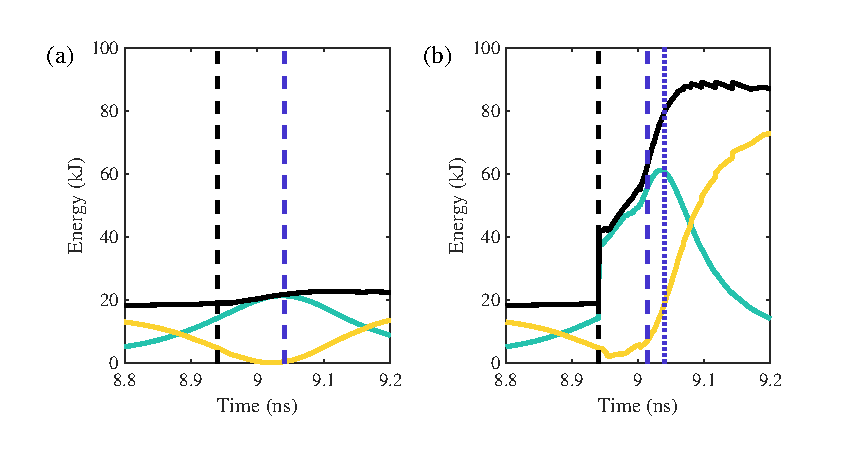
\includegraphics{figures/FurtherSims/EnergyDist.eps}
\caption{Plots showing the distribution of energy in a) an unheated capsule and b) a capsule where auxiliary heating is applied. The total energy is shown in black, with the kinetic energy in yellow and the thermal energy in teal. In both plots, the bang time is displayed by a dashed blue line, and the optimal time for auxiliary heating is a black dashed line. In b), the dotted blue line indicates the bang time for the unheated capsule (the dashed blue line in (a)), showing that the bang time occurs earlier in the implosion when heating is applied.}
\label{fig:EnergyDist}
\end{figure}

This demonstrates that adding electron energy in this way can indeed be used to improve the fusion performance of the capsule. In the following sections, this approach is applied to and investigated using four of the capsules developed in \hl{Chapter}. The key data for these capsules has been summarised in Table  \ref{tab:Heating capsules} for convenience, where they are labelled capsules A-D. In the simulations discussed in this section, the implosion is unchanged from that reported in Table \ref{tab:ThirdHarmonic} apart from the addition of the electron energy. The capsule and laser parameters are not varied. Throughout this section, the laser in the simulation - the four-pulse third-harmonic profile optimised in the previous chapter - will be referred to as the `long-pulse' laser energy, to differentiate from the hypothetical `short-pulse' laser that would be used to generate the electron beam. The phrase `heating energy' will be used to describe the added electron energy; this is varied independently of the long-pulse laser, which always has the energy described in Table \ref{tab:ThirdHarmonic}.

\begin{table}
\centering
\begin{tabular}{|c|c|c|c|c|}
\hline
Capsule label &  A & B & C & D \\ 
\hline
Size multiplier & 0.25 & 0.35 & 05 & 0.65 \\
`Long-pulse' laser energy (kJ) & 101  & 270 & 768 & 1710 \\ 
Gain & 0.030 & 0.067 & 0.19 & 0.75\\ 
\hline
  \end{tabular}
  \caption{The four capsules (labelled A-D) for which the auxilliary heating is applied to. Only the key parameters are shown; refer to Table \ref{tab:ThirdHarmonic} for full simulation details}
  \label{tab:Heating capsules}
\end{table}

\subsection{Timing of electron energy deposition}

The timing at which the heating is applied to the implosion has a large impact on the increase in fusion performance. To investigate this, simulations were performed where 4 kJ of electron energy was added to each of the four implosions being simulated, at different times around the bang-time of the unheated implosions. The results are displayed in Figure \ref{fig:HeatingTiming}. The metric used here to evaluate performance is the relative yield amplitude, which is defined here as the yield of the capsule when the heating is applied compared to the yield without auxiliary heating \footnote{Note that this is different to it's conventional usage comparing the yield when alpha self-heating is/isn't included.}.

There is a clear peak in the yield amplification as a function of time for each capsule, indicating the optimal time for the heating to be applied. This optimal time is also that displayed in Figure \ref{fig:EnergyDist}, where it can be seen that it occurs just before the minimum in kinetic energy (as the shell stops moving inwards), and just before significant amounts of fusion reactions begin. This is unsurprising: adding the energy to the hotspot prior to this point would make it harder to compress and thus reduce the density, while adding it after significant fusion has occurred will mean that the burn wave has already started to propagate, and will mean that the added energy is smaller relative to the energy of the system. Further simulations repeating this with 20 kJ of injected energy observed the same behaviour and timings as Figure \ref{fig:HeatingTiming}, suggesting these optimal values are independent of the amount of energy added.

\begin{figure}[ht]
\centering
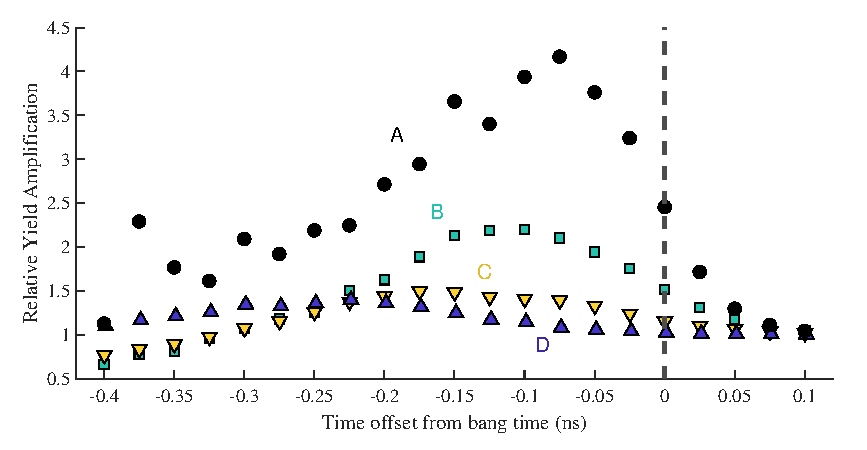
\includegraphics{figures/FurtherSims/HeatingTiming.eps}
\caption{Relative yield amplification for the capsules A-D as a function of time at which 4 kJ of electron energy is added. The capsule labels correspond to those in Table \ref{tab:Heating capsules}. The increased variation in capsule A compared to the others is likely due to the low gain of that capsule, as small changes in performance thus have a larger relative effect.}
\label{fig:HeatingTiming}
\end{figure}

\subsection{Magnitude of deposited electron energy}

Further simulations then investigated how the fusion performance varied as the amount of electron energy added was varied. The optimal time for energy deposition for each capsule from Figure \ref{fig:HeatingTiming} were identified, and the simulations then performed with between 3 to 60 kJ of electron energy deposited at this optimal time. The results can be seen in Figure \ref{fig:HeatingPower}. It can be seen that (as expected) adding more energy has a larger impact on the yield amplification, and even modest amounts of injected energy can have a significant effect. The relative yield amplification decreases as the capsule size increases; this is as expected, since 1) the larger capsules are higher energy, and thus the deposited electron energy is a smaller proportion of the capsule energy, and 2) the yield of the unheated capsule will be higher, and so a larger increase in yield is required for the same relative amplification.

\begin{figure}[ht]
\centering
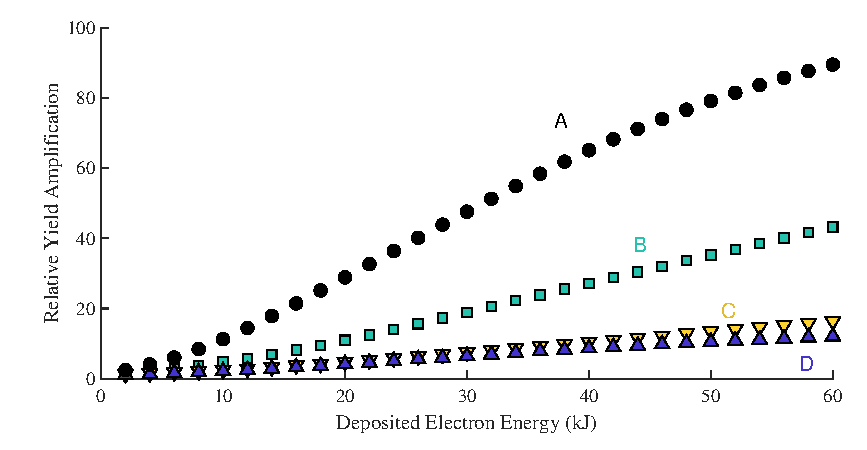
\includegraphics{figures/FurtherSims/HeatingPower.eps}
\caption{Relative yield amplification for capsules A-D as a function of the amount of deposited electron energy. The energy is injected at the optimal time for each capsule identified from Figure \ref{fig:HeatingTiming}.}
\label{fig:HeatingPower}
\end{figure}

The results are most notable for the smallest capsule (A), where 10 kJ of deposited energy gives over 10 times yield amplification, and 60 kJ amplified the yield by a factor greater than 80. Even for the largest capsule (D), 10 kJ of deposited energy is sufficient to double the yield, while 60 kJ amplifies the yield by over 12 times. This clearly shows the potential this scheme has for increasing capsule performance.

\subsection{The burning plasma parameter for heated capsules}

The (total capsule) burning plasma parameter $Q^\mathrm{{tot}}_{\mathrm{\alpha}}$ has been evaluated for the heated capsules A-D, and is displayed in Figure \ref{fig:HeatedQ}
as a function of the deposited energy \footnote{The terms were evaluated as follows: 1) the total work done $E^\mathrm{{tot}}_{\mathrm{PdV}}$ was evaluated as the sum of hotspot and shell kinetic and thermal energies just after the electron energy was added, such that the deposited energy is included in the calculation 2) the deposited alpha energy over the full capsule was used rather than the hotspot for $E_\mathrm{\alpha}$, assuming that this absorbtion is dominated by the hotspot \cite{Christopherson2018}}. These results again show the good level of performance achieved by all four capsules using auxiliary heating. While capsule D is already within the burning plasma regime, it can be seen that auxiliary heating enables both capusles B and C (which were initially sub-burning plasma) to enter it. The improvement in performance for all capsules is also clear from the improvement in $Q^\mathrm{{tot}}_{\mathrm{\alpha}}$ with heating; this is well demonstrated by capsule D which sees an improvement of almost a full order of magnitude. With the highest levels of heating it achieves a $Q^\mathrm{{tot}}_{\mathrm{\alpha}}$ approaching 10, suggesting that alpha self-heating adds almost ten times the energy to the capsule that the external compression.

\begin{figure}[ht]
\centering
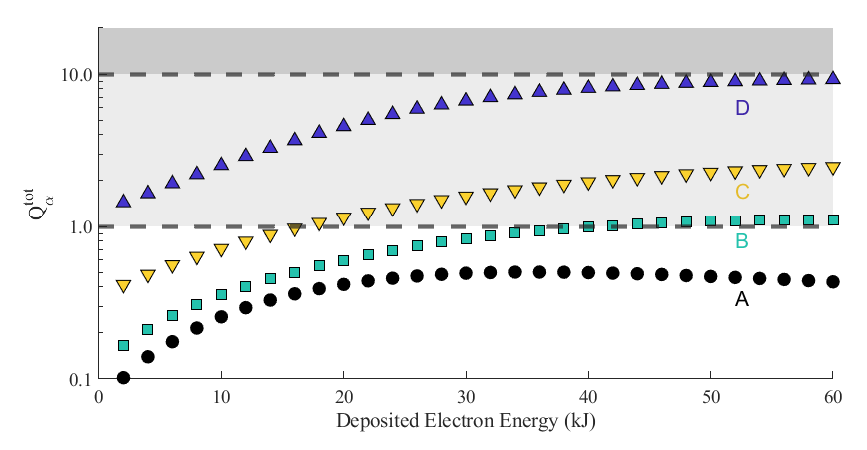
\includegraphics{figures/FurtherSims/QHeatingPlot.eps}
\caption{A log plot of the total capsule burning plasma parameter $Q^\mathrm{{tot}}_{\mathrm{\alpha}}$ vs deposited electron energy for the four capsules. Values of $Q^\mathrm{{tot}}_{\mathrm{\alpha}} = 1$ and $Q^\mathrm{{tot}}_{\mathrm{\alpha}} = 10$ are indicated.}
\label{fig:HeatedQ}
\end{figure}

\subsection{Estimating the gain of heated capsules}

Despite the challenges in calculating gain for these capsules, it is still the ultimate metric of interest for inertial fusion energy applications. Thus, the gain has been estimated using values for the relevant efficiencies from relevant literature. These efficiencies are not known to high accuracy, and thus these values are indicative only. There are two processes involved for which efficiencies must be estimated: 1) the deposition of energy into the plasma via the electron beams; and 2) the generation of the electron beams via short-pulse laser. The first of these conversion efficiencies can be taken from the Vlasov-Maxwell simulations reported by Ratan \textit{et al.} \cite{Ratan2017}, which found that the electron beams deposit electron energy with an efficiency of 18 \%.

Previous research on fast ignition has investigated electron-beam generation using short-pulse lasers, and have produced a range of estimates for the efficiencies with which such beams can be generated and transported (some examples are \cite{Ma2012, Kemp2014, Kemp2009}, and the review article \cite{Norreys2014}). For the estimates used here, two results are highlighted. The first is that of \cite{Strozzi2012}, who performed particle-in-cell simulations for an ignition scale plasma; they estimated an overall laser to electron power conversion efficiency of 52\%, which they then coupled to a hydrodynamic code for fast ignition simulations. The second is that of \cite{Tonge2009}, who also performed particle-in-cell simulations but found that as the electron beam passes through the weakly collisional background plasma a significant proportion of the energy is lost. They therefore calculated a lower efficiency of 15\% - although they also observed that this increased with both laser power, and the time for which the laser was applied. The maximum simulation time of 2.5 ps used in their work was lower than the 7 ps that the electron energy is deposited over in the Hyades simulations, iand so if this trend between deposition time and efficiency were to continue it is possible a higher effiency could be expected for this heating scheme.

In recognition of the range of values from different works, the value of 52 \% from \cite{Strozzi2012} and 15 \% from \cite{Tonge2009} have been used to provide two separate estimates of the gain. Each of these efficiencies have been combined with the 18 \% simulated coupling efficiency for electron beam energy deposition into the plasma to calculate an overall efficiency for the auxiliary heating process (capturing generation of the electron beams from short pulse laser, transport of these beams, and deposition into the plasma). The short-pulse laser energies required to cause the deposited electron energies in Figure \ref{fig:HeatingPower} were thus calculated; this was added to the `long-pulse' laser energy required for each implosion to calculate the total input energy, which was then used to calculate the gain. These two sets of estimates are displayed in Figure \ref{fig:HeatedGain}.

\begin{figure}[ht]
\centering
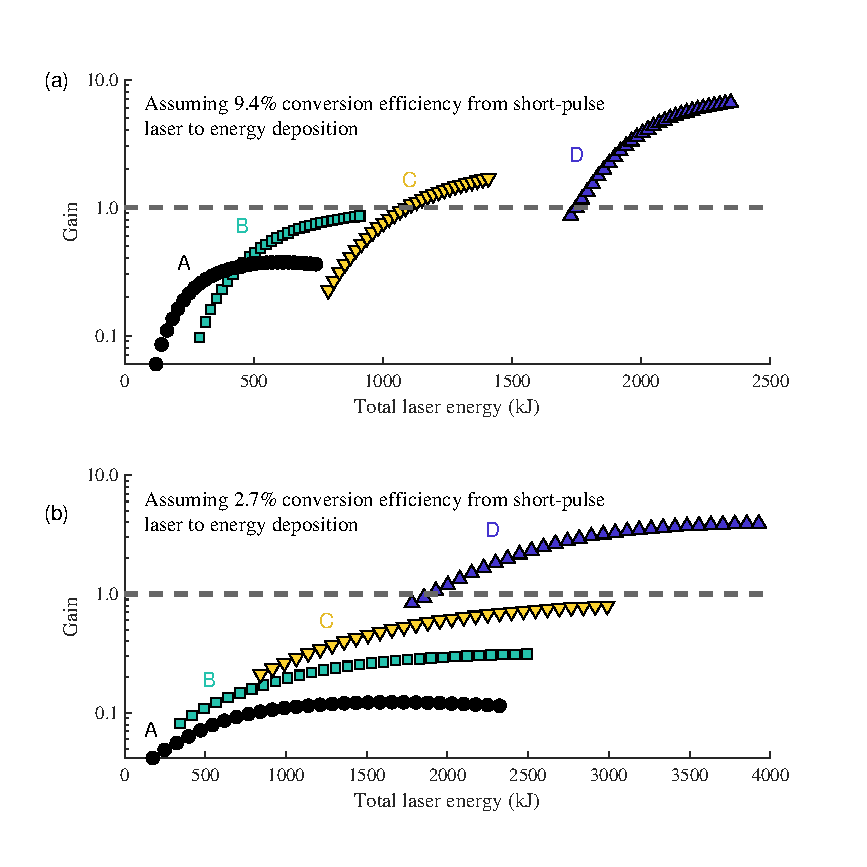
\includegraphics{figures/FurtherSims/HeatingGain.eps}
\caption{Estimated gain vs total input energy (including the `long-pulse' laser energy used to drive the implosion as reported in Table \ref{tab:Heating capsules}, and the estimated `short-pulse' laser energy required to generate the simulated amount of auxiliary heating. (a) and (b) use different estimates for the efficiency with which the heating can be generated, as indicated on the plots.}
\label{fig:HeatedGain}
\end{figure}

The general trends are the same in both figures; auxiliary heating causes an increase in gain, although this begins to saturate for larger amounts of heating energy. For the high efficiency case (a), higher gains can be achieved by using a smaller capsule with some auxiliary heating than through conventional hotspot ignition alone (as seen by the fact that lower energy capsules with a small amount of heating reach the same gains as the larger capsules for less total energy). This is unsurprising, as the 9.4 \% heating efficiency is higher than the roughly 6 \% efficiency for direct-drive laser compression \cite{Campbell2017, Goncharov2016}. For the lower efficiency case (b), direct-drive compression is higher efficiency, and so this is no longer observed. The saturation at large amounts of auxiliary heating is also not surprising; this is likely because both high density and high temperatures are required for high fusion yields, and at some point the density starts to become the limiting factor.

The results are obviously far more impressive for the high efficiency case, which predicts break-even for capsule C at around 1.1 MJ of total energy (using $\sim$ 350 kJ of short-pulse laser energy to deposit 32 kJ of electron energy into the hotspot), and gains of up to $\sim$ 3.5 for under 2 MJ of energy using capsule D. Given the observed trends, it appears likely that a capsule with size between B and C would achieve break-even for under 1 MJ of total energy. However, even in the low efficiency case, it is clear that auxiliary heating can still be a useful tool to improve the performance of a capsule, and capsule D can be seen to achieve break-even for under 2 MJ using this technique.

\subsection{Comparison with previous simulated and experimental results}

The results presented for capsules A-D can be compared to a range of previous results. Simulations were previously performed to estimate the impact such a scheme may have on indirectly-driven targets, which were presented in \cite{Norreys2021}. This was based on the NIF shot N160421, with a low convergence ratio and a drive energy of $\sim 800$ kJ. The greater efficiency of direct-drive implosions results in an approximately five-fold increase in the amount of energy deposited in the hotspot \cite{Campbell2017, Goncharov2016}, which means that such a capsule should be roughly equivalent to an implosion in this work with an energy of around 150 kJ. There are some minor differences between these works; the indirect-drive results demonstrate less dependence on the time at which the heating is applied, and a lower level of amplification than would be expected based on the results presented here (some differences should be expected due to the use of a different code, XRAGE, for the indirect drive simulations, and for the differences in the base implosions - with the indirect-drive implosion having significantly lower yield). Despite this the results are broadly similar between the two works, with similar trends observed in both the direct and indirect-drive simulations.

The fusion performance of capsule B is also comparable to that of NIF shots N190918, N191007, and N191110 (the capsules with record inertial fusion yields when this work was first performed \cite{Zylstra2021}), although these shots targeted higher convergence ratios over 25. These NIF shots produced neutron yields ranging from \num{0.75e16} to \num{2e16} (compared to \num{0.8e16} for capsule B without auxiliary heating) and fuel kinetic energies of $\sim$15~kJ (also similar to capsule B), for $\sim$1.9~MJ of indirect drive input energy. These shots led to predictions that laser energies of $\sim$3~MJ \cite{Zylstra2021} may have been required to achieve MJ-level yields (other predictions thought energies of up to $\sim$5~MJ may be required \cite{Zylstra2021, Cheng2021}). However, extrapolating the auxiliary heating results presented for capsule B to these implosions suggested that MJ-level yields could be achieved for a total of 2.3 MJ \footnote{This was estimated by taking the 56 kJ yield of N191110, and assuming based on implosion B in Figure \ref{fig:HeatingPower} that a yield amplification of twenty times could be achieved for 32 kJ of auxiliary heating, which would require less than 350 kJ of short-pulse laser energy assuming a conversion efficiency of 9.6 \%.}. This highlights how such a heating scheme could potentially be used to improve the performance of real NIF shots. These results could also be extrapolated for the 1.3 MJ yield shot N210808. This has a yield between those of capsules C and D; applying a similar extrapolation suggests that this yield could be doubled for only 10 kJ of deposited energy. These are illustrative examples only, but serve to demonstrate how this technique could be applicable more widely than just for the low-instability shots discussed here.

\subsection{Auxiliary heating of high gain capsules}
Auxiliary heating was also later applied to three of the alternative laser drivers implosions. The main purpose of this was to see the effect of auxiliary heating on high gain capsules; auxiliary heating helps the capsule to achieve ignition without adding more fuel, and thus it is likely that for better performing capsules the increase in performance would be more moderate. It also allowed the combination of these technologies to be assessed. These simulations were performed by summer students Tat Li and Eugene Kim, under my supervision.

Three capsules were used: the 0.5 and 0.65 size two-colour implosions, and the 0.5 size ArF implosion \footnote{These simulations were performed a year after the capsules were first optimised, and used the updated HYADES version 01.12.05 compared to version 01.12.03 for the original simulations. Rerunning the unheated input decks using this new version resulted in a slightly increased yield. This explains why the gain at low heating levels in Figure \ref{fig:TwoColourAux} is still higher than that reported in Table \ref{tab:Heating two colour capsules}.}.  These capsules are labelled E-G in Table \ref{tab:Heating two colour capsules}. The auxiliary heating was simulated exactly as described in the previous sections, and the optimal timing for the heating was identified as outlined previously, before the amount of deposited energy was varied. The results are shown in Figure \ref{fig:TwoColourAux}.

\begin{table}
\centering
\begin{tabular}{|c|c|c|c|}
\hline
Capsule label &  E & F & G  \\ 
\hline
Laser driver & \multicolumn{2}{c|}{Two-colour} & ArF \\ 
\hline
Size multiplier & 0.5 & 0.65 & 0.5 \\
\hline
`Long-pulse' laser energy (MJ) & 1.69  & 2.10 & 1.91 \\ 
Gain & 4.0 & 15.5 & 17.3 \\ 
\hline
  \end{tabular}
  \caption{The three high gain implosions (labelled E-G) for which the auxilliary heating is applied to. Full details can be found in Table \ref{tab:TwoColourTable}.}
  \label{tab:Heating two colour capsules}
\end{table}

\begin{figure}[ht]
\centering
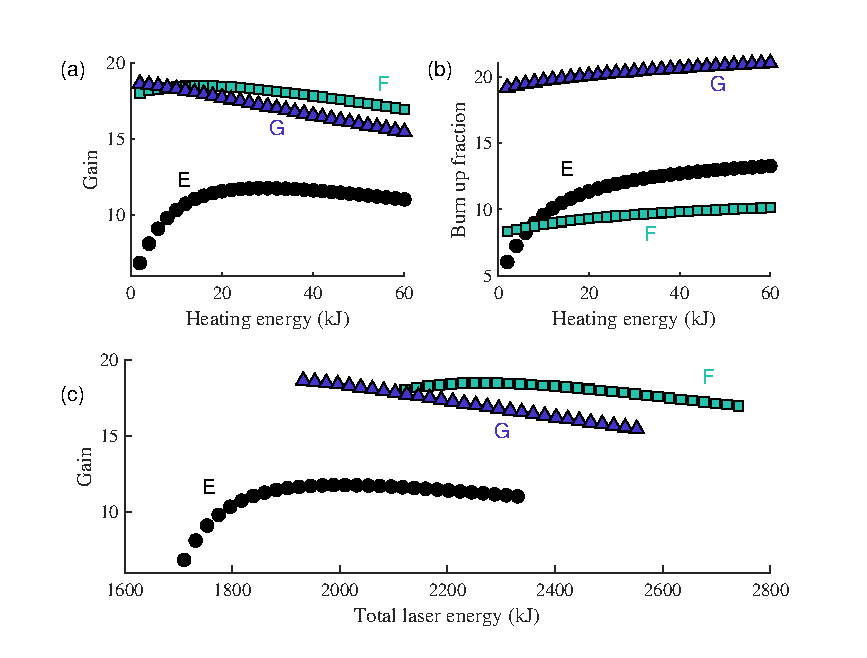
\includegraphics{figures/FurtherSims/TwoColourAux.eps}
\caption{Auxiliary heating for two two-colour implosions (E and F) and one ArF implosion (G). In (a), the estimated gain (assuming a 9.4 \% heating efficiency) is plotted as a function of the heating energy. In (b), the burn-up fraction of the three implosions versus heating energy is displayed. (c) shows the estimated gain, as a function of the total estimated input energy.}
\label{fig:TwoColourAux}
\end{figure}

As expected, it was found that for higher gain capsules, the auxiliary heating is much less beneficial. The 0.5 size capsule has the lowest base gain, and it can be seen that adding electron energy allows the gain to increase by a moderate amount, but after this it actually begins to decrease. This corresponds to a scenario where the additional fusion reactions generated by the increase in energy no longer compensate for the additional cost. This is not unexpected - this capsule has already achieved the conditions necessary for a large amount of fusion reactions to occur, and thus the amount of electron energy deposited (as a fraction of the hotspot energy) is much less significant than for the previous capsules.

As the yield of the unheated implosion further increases, this effect becomes even more dramatic. The 0.65 size two-colour capsule sees an even smaller fractional increase in performance, and less electron energy can be added before the gain begins to decrease. For the ArF capsule, adding electron energy offers no benefit and the gain decreases from the start. This is despite the unheated gain being very similar to that for the 0.65 size two-colour capsule. The reason for this is that the ArF capsule is smaller (the energy is the same due to the higher laser power), and has a much higher burn up fraction (as shown in Figure \ref{fig:TwoColourAux} (b)). The unheated ArF capsule is therefore further along it's ignition curve - it is already igniting very well, and is close to the maximum possible yield for this capsule. The two-colour capsule is larger, with more fuel and a higher saturation gain, and thus the performance can be further increased compared to the ArF capsule.

\section{Optimisation and heating of high areal-density capsules}
The implosions A-D (and the high gain capsules) are each implosions that were originally optimised for high gain, in the absence of auxiliary heating. However, it may be that if the conventional implosion and the auxiliary heating were considered together, there may be alternative implosions that would return a higher gain once the heating is applied.

This would add significant complexity to the optimisation, which makes it infeasible to explore without further development. However, it is possible to predict the form of such an implosion. Auxiliary heating allows the temperature of the capsule to be significantly increased, but the areal density is unchanged. As such, it was suggested that if an implosion could be developed with a higher areal density (at the expense of a lower temperature and yield), then once auxiliary heating is applied to increase the ion temperature the resulting yield/gain may be higher than if a capsule optimised for yield was heated.

To explore this, a further two optimisations were performed. This followed the exact procedure as before, but the implosions were optimised to produce a capsule with the maximum possible areal density (i.e. the areal density of DT within both hotspot and shell), rather than yield. I again produced the changes to the code necessary to enable this, and then supervised a summer student, Tat Li, in performing the optimisation. The resulting `optimal areal density' implosions are included in Table \ref{tab:Optimal Areal Density}, along with the corresponding `high gain' version. Auxilliary heating was then applied, first identifying the optimal timing for the capsules, and then varying the deposited energy. The resulting gains (assuming the optimistic 9.4\% conversion efficiency for the heating) is then displayed in Figure \ref{fig:OptimisedRhoR}.


\begin{table}
\centering
\begin{tabular}{|c|c|c|c|c|c|c|}
\hline
Laser driver & \multicolumn{2}{c|}{Third harmonic} & \multicolumn{2}{c|}{ArF} \\ 
\hline
Size multiplier & \multicolumn{2}{c|}{0.5} & \multicolumn{2}{c|}{0.5} \\ 
\hline
Optimised for & Gain & $\rho R$ & Gain & $\rho R$  \\
\hline
Laser energy (MJ)  & 0.77 & 0.80 & 1.91 & 2.16 \\ 
Gain (original) &  0.19 & - & 17.3 & -\\ 
Gain (at time of work) &  0.19 & 0.12 & 18.7 & 24.7\\ 
Areal Density (\unit{\gram\per\centi\meter\squared}) & 0.71 & 0.76 & 1.04 & 1.30\\
Convergence ratio  & 16.0 & 15.9 & 15.9 & 15.9 \\ 
IFAR  & 29.7 & 23.2 & 10.5 & 9.0 \\ 
Implosion velocity (km/s)  & 399.6 & 358.1 & 398.9 & 361.9\\ 
Pulse 2 switch on time (ns)  & 2.60 & 3.60 & 3.50 & 4.20\\ 
Pulse 3 switch on time (ns) & 5.60 & 6.80 & 7.50 & 9.20\\ 
Pulse 4 switch on time (ns)  & 6.80 & 8.20 & 9.25 & 11.00 \\ 
Laser switch off time (ns)  & 11.00 & 12.60 & 12.25 & 14.40 \\ 
Vapour/liquid boundary (\si[per-mode=symbol]{\milli\meter})  & 1.305 & 1.290 & 1.210 & 1.150\\ 
Liquid/CD boundary (\si[per-mode=symbol]{\milli\meter})  & 1.3950 & 1.390 & 1.340 & 1.340\\ 
Outer radius (\si[per-mode=symbol]{\milli\meter})  & 1.425 & 1.425 & 1.425 & 1.425\\ 
Vapour density (\si[per-mode=symbol]{\milli\gram\per\centi\meter\cubed})  & 1.050 & 1.200 & 1.030 & 1.405\\
\hline
  \end{tabular}
  \caption{Newly optimized `optimal areal density' implosion simulation parameters, for the 0.5 size third-harmonic and ArF implosions. The data for the original `optimal gain' implosions have been included for comparison.}
  \label{tab:Optimal Areal Density}
\end{table}

\begin{figure}[ht]
\centering
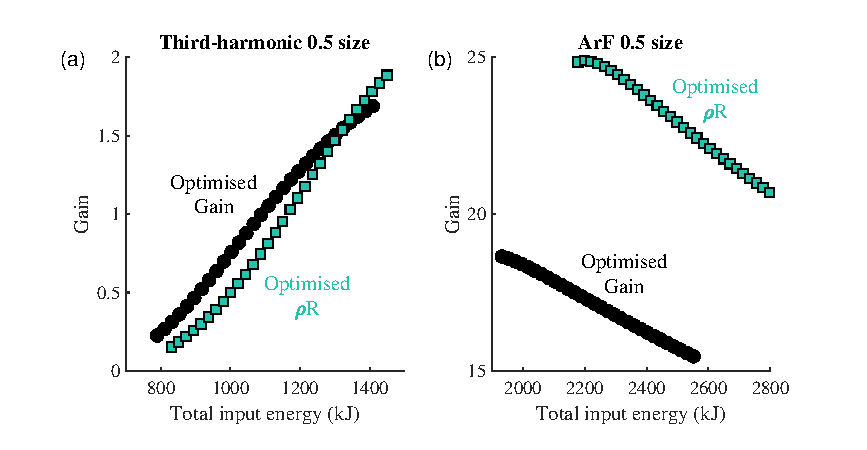
\includegraphics{figures/FurtherSims/OptimisedRhoR.eps}
\caption{Estimated gain vs total input energy for the 0.5 sized capsules optimised for gain (black) and areal density (teal), for a third-harmonic (a) and ArF (b) laser driver.}
\label{fig:OptimisedRhoR}
\end{figure}

The gain for the smaller of the two capsules, seen in Figure \ref{fig:OptimisedRhoR}, behaved as predicted. It can be seen that at low amounts of heating energy the `optimal gain' capsule outperforms the `optimal areal density' version, as expected. However, as the heating energy is increased further, the `optimal areal density' capsule begins to perform better, producing a higher gain that the `optimal gain capsule'. The `optimal gain' capsule begins to saturate earlier - this makes sense, since it has a lower areal density and a higher temperature, and so the temperature stops being the limiting factor much earlier than for the `optimal areal density' version.

A number of factors mean that the data in Figure \ref{fig:OptimisedRhoR} is more complicated to analyse. Firstly, the optimisation procedure in this case gave an `optimal areal density' capsule at a higher laser drive than the `optimal gain' capsule (recall that this is the optimal capsule for a given radius - and not necessarily a given drive energy). The higher laser drive meant that the capsule gain was also higher, hindering useful comparison between the two capsules \footnote{This also indicates, as explained earlier, that the optimisation is not exhaustive - as there is clearly a design for this capsule radius with a higher gain than that initially optimised.}. As seen in Figure \ref{fig:OptimisedRhoR} (b), the gain is therefore higher for all amounts of deposited energy. Secondly, the much higher gain of this capsule means that the auxiliary heating in both cases does not lead to significant increases in gain, as discussed in SECTION. However, qualitative differences are still visible - although increases in gain are not seen, it is clear that `optimal areal density' capsule is still improved more by the heating (despite the higher gain and laser energy), as indicated by the fact that the gain is relatively constant at low energies as opposed to decreasing (as seen for the `optimal gain' capsule). This is confirmed by the relative yield amplification, which shows a greater relative increase for the `optimal areal density' capsule at low energies.

\subsection{Limitations and suggested future direction}

As stated at the start, the simulations presented here are an initial investigation of the effects of such a heating scheme. They do not simulate the scheme itself, and thus high accuracy should not be expected. However, they indicate a promising level of performance, and suggest that further investigation of this heating process in more detail could be useful. This includes simulations of the full heating process using Vlasov-Maxwell and particle-in-cell codes, along with multi-scale modelling. These are directions that are under further investigation within our group.

Another limitation of this work is the lack of accuracy to which the efficiencies for the generation and transport of the electron beams are known. These efficiencies are vital for accurate estimates of the implosion gain, and so should be determined if such a scheme is to be pursued.

A final potential limitation of this approach are the high short-pulse laser energies required. These are significantly higher than the short-pulse energies available at current facilities, and are similar to those necessary for fast-ignition schemes \cite{Strozzi2012}. Again, this an an initial investigation of this approach, which is focussed on whether such a scheme may be worthwhile than the practical aspects of achieving it. However, recent developments such as plasma beam combiners \cite{Kirkwood2018,Kirkwood2018a} may offer a route through which short-pulse laser energies could be increased in the future to the levels required \cite{KirkwoodPersonalComm}. Plasma beam combiners utilise non-linear scattering interactions within plasma-based optical components to produce a single laser output from multiple input beams, achieving a much higher intensity than is possible with conventional optics. It is hoped that continued development of this approach, and of short-pulse laser technology more generally, may enable the energies required for such a scheme.

\subsection{Subsequent developments of the auxiliary heating technique}
Since this work was performed, there have been further developments in understanding this technique which affect how it would be applied. This is not my work (it was performed by Jordan Lee, Rusko Ruskov, and Heath Martin) - but it was performed following the promising results shown here, and is mentioned for completeness and improved understanding of the technique.

In the previous discussions, the heating scheme was assumed to require two overlapping electron beams. This was the setup proposed in \cite{Ratan2017}; the highest growth rates for the instabilities was seen at the overlap of these beams, and it was expected that this would therefore be where the most significant heating occurred. Having two beams in this way allowed for control over where the energy would be deposited. However, further research instead discovered that there is no benefit to using two beams - the heating growth quickly saturates, and thus two beams provides no benefit over one. The heating occurs along the beam according to the plasma conditions, and thus the position of the energy deposition cannot be controlled in this way.

Simulations of an electron beam incident on the capsule around the bang-time found that the vast majority of the energy is deposited at the edge of the hotspot. The electron beam passes through the cold, dense shell with very little absorption, but is absorbed effectively as soon as it reaches the high temperature hotspot. This is different to the simulations here, where the energy deposition was assumed to be uniform over the central region in the simulation. However, updated versions of these HYADES simulations (performed by Jordan Lee) accounted for this, instead depositing the electron energy in a thin shell (of appropriate thickness) around the hotspot. It was found that these actually slightly improved the performance\footnote{It is suggested that this is because the material at the edge of the hotspot is likely slightly higher density but colder - and thus the heating has more of an effect}. Of course, this assumes that the heating is spherical, whereas in fact this would only occur in the direction of the beam - 2D simulations are required to investigate this in further detail.

\section{Conclusions}
This chapter expanded upon the results of the previous chapter in a variety of different ways. Firstly, two potential limitations of the previous work were explored. The impact of the EOS used to describe the wetted-foam layer was investigated. \hl{Comment}. Secondly, surrogate `hydrodynamic equivalent' implosions were optimised for a number of capsules, and displayed equivalent hydrodynamic performance to the main implosions. This provides a way that the results of the previous chapter (and the low-instability nature of the regime) could be explored in room-temperature experiments.

The impact of alternative laser drivers on implosions in this regime were then explored. It was demonstrated that switching from a third-harmonic Nd:glass laser to a higher frequency (ArF in this work) could lead to substantial increases in fusion performance at a given energy. A `two-colour' laser sequence was also proposed, which would allow some of the performance benefits of higher frequency laser energies to be obtained, while allowing the bulk of the energy to be provided by the more mature Nd:glass technology.

Finally, the effect of auxiliary heating on a number of these implosions was simulated. It was found that such a technique could potentially be used to significantly improve the fusion performance of a range of capsules. The increase on gain was also estimated to be significant, but this is highly dependent on how efficiently electron beams can be generated and their energy deposited into the hotspot. Further simulation identified that the impact is significantly decreased as the yield of the unheated implosion increases, suggesting that auxiliary heating is more useful for helping sub-ignition capsules to ignite rather than amplifying the gain of already well-performing capsules. 





